\documentclass[conference]{IEEEtran}
\IEEEoverridecommandlockouts
% Based on the IEEE conference template (Overleaf: "IEEE Conference Template").
\usepackage{cite}
\usepackage{amsmath,amssymb,amsfonts}
\usepackage{algorithm}
\usepackage{algorithmic}
\usepackage{graphicx}
\usepackage{textcomp}
\usepackage{xcolor}
\usepackage{booktabs}
\usepackage{url}
\usepackage{tikz}
\usetikzlibrary{arrows.meta,positioning,fit,backgrounds}
\usepackage{pgfplots}
\pgfplotsset{compat=1.18}
\def\BibTeX{{\rm B\kern-.05em{\sc i\kern-.025em b}\kern-.08em
    T\kern-.1667em\lower.7ex\hbox{\sc e}\kern-.125emX}}

% Shared bar-chart style for the benchmark figures
\pgfplotsset{benchbar/.style={
    ybar, width=\columnwidth, height=3.9cm, bar width=13pt,
    symbolic x coords={XDP,TC,TC+FIB,Kernel,OVS}, xtick=data,
    ymin=0, enlarge x limits=0.13, axis lines*=left,
    ymajorgrids, grid style={gray!25},
    nodes near coords, every node near coord/.append style={font=\scriptsize},
    tick label style={font=\footnotesize}, label style={font=\footnotesize}}}

\begin{document}

\title{In-Kernel Programmable Data Planes for SDN:\\
An eBPF/XDP Gateway with Stateful Firewalling and\\
L4 Load Balancing Compared with Open vSwitch}

\author{\IEEEauthorblockN{Author Name}
\IEEEauthorblockA{\textit{Department of Computer Science and Engineering} \\
\textit{University Name}\\
City, Country \\
email@example.com}}

\maketitle

\begin{abstract}
Software-Defined Networking (SDN) classically separates a controller from
switches that execute OpenFlow match--action tables. Cloud-native platforms
increasingly move this data plane into the operating-system kernel using the
extended Berkeley Packet Filter (eBPF) and the eXpress Data Path (XDP). This
paper designs, implements and evaluates such a data plane for a gateway that
combines a stateful firewall, a Layer-4 (L4) load balancer with destination
and source network address translation (DNAT/SNAT), and per-flow telemetry.
A single verified eBPF pipeline is attached either at the XDP or at the
Traffic Control (TC) hook; a Python control plane programs it at runtime
through pinned BPF maps, exposes a REST interface and expires idle connections
in the manner of OpenFlow idle timeouts. We formalize rule matching, backend
selection, incremental checksum updates and connection expiry, and we verify
the implementation with 69 automated tests, including kernel-level
packet tests that check every rewritten checksum, and with end-to-end Mininet
scenarios. Against an Open vSwitch (OVS) baseline programmed with equivalent
OpenFlow~1.3 rules, both systems forward and filter correctly and spread load
evenly ($\chi^2$ test, $p \ge 0.25$), but only the eBPF data plane supports
connection tracking and backend draining. On virtual Ethernet links the eBPF
pipeline reaches 2.4--3.0~Gbit/s of TCP throughput and 139--148~kpps for
64-byte packets, 21--26\% below plain kernel routing, whereas OVS stays within
2\% of it. We explain why veth links mask XDP's driver-level advantage and
identify the conditions under which the in-kernel design is expected to pay
off.
\end{abstract}

\begin{IEEEkeywords}
software-defined networking, eBPF, XDP, programmable data plane, load
balancing, stateful firewall, Open vSwitch, Mininet
\end{IEEEkeywords}

%=====================================================================
\section{Introduction}
%=====================================================================
SDN decouples the control plane, which decides how traffic should be handled,
from the data plane, which applies those decisions packet by packet
\cite{kreutz2015sdn,feamster2014road}. OpenFlow \cite{mckeown2008openflow}
standardized this split: a controller installs prioritized match--action
entries into the flow tables of switches such as Open vSwitch (OVS)
\cite{pfaff2015ovs}. The model is expressive for stateless forwarding, but
richer network functions---stateful firewalls, connection-aware load
balancers, fine-grained telemetry---require either protocol extensions or
processing outside the switch pipeline.

Cloud-native infrastructures have taken a different path. eBPF allows verified
programs to be loaded into a running Linux kernel and attached to networking
hooks, and XDP runs such programs in the network driver before the kernel
allocates its packet structure \cite{hoiland2018xdp,vieira2020ebpf}.
Production systems such as Cilium for Kubernetes networking
\cite{cilium} and Katran for L4 load balancing \cite{katran} implement their
data planes this way. The controller--switch boundary of SDN thus becomes a
boundary between a user-space agent and kernel tables (BPF maps).

This paper studies that transition on a concrete, fully implemented system.
Our contributions are:
\begin{enumerate}
\item A single eBPF pipeline, attachable at the XDP or TC hook, that parses
Ethernet/VLAN/ARP/IPv4/TCP/UDP/ICMP, enforces a stateful firewall over
5-tuple and MAC rules, load-balances connections to a virtual IP (VIP) with
DNAT/SNAT, and maintains per-flow telemetry (Section~\ref{sec:method}).
\item A control plane that loads the program with libbpf, programs it at
runtime through a CLI and a REST API, and expires connection state with idle,
FIN and hard timeouts analogous to OpenFlow timeouts.
\item A formal model of the rule-matching order, backend selection, NAT
checksum maintenance and connection expiry, which is exactly the logic the
implementation executes (Section~\ref{sec:model}).
\item An evaluation against plain kernel routing and an OVS/OpenFlow~1.3
baseline with equivalent policy, including correctness tests, load
distribution analysis and throughput, packet-rate and latency measurements
(Sections~\ref{sec:setup}--\ref{sec:results}).
\end{enumerate}

%=====================================================================
\section{Related Work}
%=====================================================================
\textit{SDN and OpenFlow.} Kreutz \textit{et al.}\ survey the SDN
architecture and its data-plane abstractions \cite{kreutz2015sdn}; Feamster
\textit{et al.}\ trace its intellectual history \cite{feamster2014road}.
OpenFlow \cite{mckeown2008openflow} defines the match--action switch model
that OVS \cite{pfaff2015ovs} implements with a user-space slow path and a
kernel flow cache. P4 \cite{bosshart2014p4} generalizes the data plane to
protocol-independent pipelines, mainly targeting hardware switches.

\textit{eBPF and XDP.} H{\o}iland-J{\o}rgensen \textit{et al.}\ present the
design of XDP and show drop and forwarding rates of tens of millions of
packets per second per core on physical NICs \cite{hoiland2018xdp}. Vieira
\textit{et al.}\ provide a tutorial survey of eBPF and XDP
\cite{vieira2020ebpf}. Miano \textit{et al.}\ report on building complex
network services from eBPF programs and on the limits imposed by the verifier
\cite{miano2018creating}, and Scholz \textit{et al.}\ quantify the performance
of eBPF-based packet filtering in Linux \cite{scholz2018filtering}.

\textit{Software load balancers.} Maglev \cite{eisenbud2016maglev} is a
distributed software L4 load balancer that uses consistent hashing and
connection tracking; Katran \cite{katran} realizes a similar design with XDP.
Our load balancer follows the same principles---hash-based backend selection
with per-connection stickiness---but in a compact, verifiable form suitable
for direct comparison with an OpenFlow \texttt{select} group.

\textit{Emulation.} Mininet \cite{lantz2010mininet} emulates SDN topologies
with network namespaces and virtual Ethernet (veth) pairs. Because emulated
hosts share one kernel, an eBPF program attached inside Mininet is the real
kernel program, which makes Mininet suitable for functional validation;
its performance limits are discussed in Section~\ref{sec:threats}.

Compared with these works, we contribute an end-to-end, open
implementation that combines firewalling, load balancing and telemetry in one
eBPF pipeline at two hook points, and we evaluate it side by side with an
OpenFlow baseline implementing the same policy.

%=====================================================================
\section{Problem Scenario and System Model}
\label{sec:model}
%=====================================================================
\subsection{Scenario}
A gateway connects a client subnet $\mathcal{C}=\{c_1,\dots,c_4\}$
(10.0.1.0/24) and a backend subnet $\mathcal{S}=\{s_1,\dots,s_4\}$
(10.0.2.0/24). A service is published at the VIP $v=10.100.0.1$, port 80, and
must be served by the backends. The gateway must (i) forward all inter-host
traffic, (ii) enforce operator-defined allow/drop rules, (iii) distribute new
connections to the VIP across healthy backends while keeping each connection
on one backend, (iv) let operators drain a backend, and (v) export packet and
byte counters. Rules and backend pools change at runtime without reloading
the data plane.

\subsection{System Model}
Fig.~\ref{fig:arch} shows the architecture. Every host has a dedicated veth
link to the gateway (\textit{routed access}: /32 host routes and proxy ARP),
so every packet between any two hosts traverses the gateway data plane. The
data plane is a set of kernel functions sharing nine BPF maps; the control
plane reads and writes the same maps through the \texttt{bpf()} system call.

\begin{figure}[t]
\centering
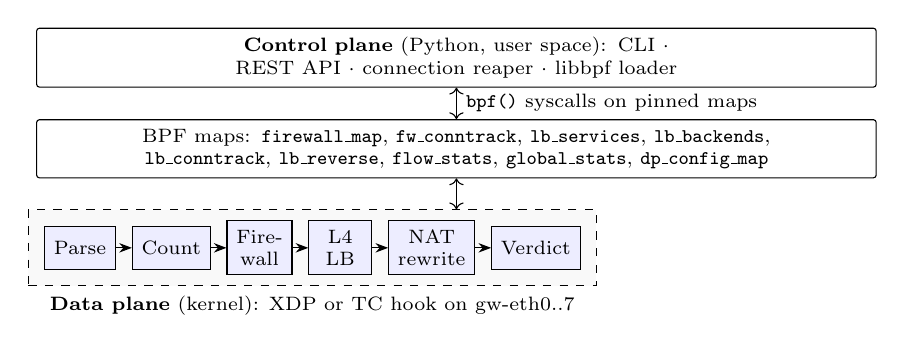
\begin{tikzpicture}[font=\scriptsize, node distance=2mm,
  box/.style={draw, rounded corners=1pt, align=center, minimum height=5mm, fill=white},
  stage/.style={draw, fill=blue!7, minimum height=5.5mm, minimum width=8mm, align=center},
  arr/.style={-{Stealth[length=1.6mm]}}]
\node[box, text width=0.86\columnwidth] (cp) {\textbf{Control plane} (Python, user space):
  CLI $\cdot$ REST API $\cdot$ connection reaper $\cdot$ libbpf loader};
\node[box, below=4mm of cp, text width=0.86\columnwidth] (maps)
  {BPF maps: \texttt{firewall\_map}, \texttt{fw\_conntrack}, \texttt{lb\_services},
   \texttt{lb\_backends},\\ \texttt{lb\_conntrack}, \texttt{lb\_reverse},
   \texttt{flow\_stats}, \texttt{global\_stats}, \texttt{dp\_config\_map}};
\node[stage, below=6mm of maps.south west, anchor=north west, xshift=1mm] (p) {Parse};
\node[stage, right=of p] (t) {Count};
\node[stage, right=of t] (f) {Fire-\\wall};
\node[stage, right=of f] (l) {L4\\LB};
\node[stage, right=of l] (n) {NAT\\rewrite};
\node[stage, right=of n] (v) {Verdict};
\draw[arr] (p) -- (t); \draw[arr] (t) -- (f); \draw[arr] (f) -- (l);
\draw[arr] (l) -- (n); \draw[arr] (n) -- (v);
\begin{scope}[on background layer]
\node[draw, dashed, fill=gray!5, inner sep=2mm, fit=(p)(v),
  label={[font=\scriptsize]below:\textbf{Data plane} (kernel): XDP or TC hook on gw-eth0..7}] (dp) {};
\end{scope}
\draw[arr, <->] (cp) -- node[right] {\texttt{bpf()} syscalls on pinned maps} (maps);
\draw[arr, <->] (maps.south) -- (maps.south |- dp.north);
\end{tikzpicture}
\caption{Architecture: a user-space control plane programs a kernel data
plane through shared BPF maps.}
\label{fig:arch}
\end{figure}

\subsection{Flows and Rules}
A packet $x$ carries the flow key
\begin{equation}
f(x) = (s, d, p_s, p_d, \pi),
\end{equation}
with source and destination addresses $s,d$, ports $p_s,p_d$ (zero for
protocols without ports) and protocol $\pi$. The reverse key is
$\bar f = (d, s, p_d, p_s, \pi)$. A firewall rule is a key $k$ in the rule
table $\mathcal{R}$ with an action $a(k)\in\{\textsc{allow},\textsc{drop}\}$,
where a zero field denotes a wildcard. MAC rules use the key
$(\mathrm{mac}_s, \mathrm{mac}_d)$ with $\mathrm{mac}_d$ optionally wildcarded.

Let $m_1,\dots,m_9$ be the masking functions, ordered from most to least
specific:
\begin{equation}
\begin{aligned}
&m_1{:}\,(\mathrm{mac}_s,\mathrm{mac}_d),\;\; m_2{:}\,(\mathrm{mac}_s,*),\;\;
 m_3{:}\,(s,d,p_s,p_d,\pi),\\
&m_4{:}\,(s,d,*,p_d,\pi),\;\; m_5{:}\,(s,d,p_s,*,\pi),\;\;
 m_6{:}\,(s,d,*,*,\pi),\\
&m_7{:}\,(s,d,*,*,*),\;\; m_8{:}\,(s,*,*,*,*),\;\; m_9{:}\,(*,d,*,*,*),
\end{aligned}
\end{equation}
where $m_3$--$m_5$ apply only to TCP and UDP. The matched action is that of
the first matching key,
\begin{equation}
\label{eq:match}
A(x) = a\big(m_{i^*}(x)\big),\quad
i^* = \min\{\, i : m_i(x) \in \mathcal{R} \,\},
\end{equation}
and $A(x)=\textsc{none}$ if no key matches.

\subsection{Stateful Admission}
Let $\mathcal{T}_{fw}$ be the set of tracked firewall flows, $\mathcal{T}_{rev}$
the set of load-balancer reply keys, and $\delta$ the default action. With
connection tracking enabled, a flow is \textit{established} iff
$E(f) = \mathbb{1}\big[f \in \mathcal{T}_{fw} \lor \bar f \in \mathcal{T}_{fw}
\lor f \in \mathcal{T}_{rev}\big]$, and an IPv4 packet is admitted iff
\begin{equation}
\label{eq:adm}
\mathrm{adm}(x) =
\begin{cases}
0 & A(x) = \textsc{drop},\\
1 & A(x) = \textsc{allow} \;\lor\; \delta=\textsc{allow},\\
E(f) & \text{otherwise}.
\end{cases}
\end{equation}
Admitted flows are inserted into (or refresh) $\mathcal{T}_{fw}$. ARP packets
are subject only to MAC rules, so address resolution cannot be broken by an
IP policy.

\subsection{Load-Balancing Model}
A service $\sigma=(v,p_v,\pi)$ owns an ordered backend pool
$B_\sigma=(b_0,\dots,b_{n-1})$, $n \le 16$, where each backend $b_j$ has an
address, a port and an activity flag $\alpha_j\in\{0,1\}$. For a new
connection, the gateway computes a hash $h(f)$ (Bob Jenkins' \textit{jhash}
final mix over $s$, $d$ and the port/protocol word), lets
$r = h(f) \bmod n$, and selects
\begin{equation}
\begin{aligned}
j^*(f) &= (r + k^*) \bmod n, \\
k^* &= \min\{\, k \in [0,n) : \alpha_{(r + k) \bmod n} = 1 \,\}.
\end{aligned}
\label{eq:select}
\end{equation}
If no backend is active, the packet is dropped. The choice is stored in the
connection table $\mathcal{L}$ as $\mathcal{L}[f]=(b_{j^*}, j^*)$ and reused
for every later packet of $f$ as long as $\alpha_{j^*}=1$ and the backend's
address is unchanged; otherwise a new backend is selected. If $h$ is uniform,
the number of connections $N_j$ received by each of $n$ active backends out of
$N$ satisfies $\mathbb{E}[N_j]=N/n$, which we test with Pearson's statistic
\begin{equation}
\chi^2 = \sum_{j=0}^{n-1} \frac{(N_j - N/n)^2}{N/n}, \qquad
\text{d.o.f.} = n-1.
\label{eq:chi2}
\end{equation}

\subsection{Address Translation}
For a client flow $f=(c,v,p_c,p_v,\pi)$ assigned to backend $b=(a_b,p_b)$, the
forward packet is rewritten by DNAT,
$T_D(f)=(c,a_b,p_c,p_b,\pi)$, and the reverse-NAT table records the key of
the expected reply, $\mathcal{T}_{rev}[(a_b,c,p_b,p_c,\pi)] = (v,p_v)$. A reply
matching this key is rewritten by SNAT to $(v,c,p_v,p_c,\pi)$, so the client
only ever observes the VIP.

\subsection{Incremental Checksum Maintenance}
Rewriting addresses and ports invalidates the IPv4 header checksum and the
TCP/UDP checksum, whose pseudo-header covers both addresses. Recomputing them
over the packet costs $O(L)$ for a packet of length $L$. Instead we use the
incremental update of RFC~1624 \cite{rfc1624}: if 16-bit words $m_i$ change
to $m_i'$, the new checksum is
\begin{equation}
HC' = \sim\!\Big(\sim\!HC + \sum_i \sim m_i + \sum_i m_i'\Big),
\label{eq:csum}
\end{equation}
in ones'-complement arithmetic \cite{rfc1071}, which is $O(1)$. For the IPv4
header the changed words are the two halves of one address; for the L4
checksum they are the address (via the pseudo-header) and the port. Because
TCP and UDP headers both begin with the 32-bit word $(p_s,p_d)$, the address
and the port word are passed to a single \texttt{bpf\_csum\_diff} call over
8~bytes. A UDP checksum of zero (``not computed'') is left unchanged, and a
computed result of zero is transmitted as \texttt{0xFFFF}.

\subsection{Connection Expiry}
Each tracked entry $e$ stores its creation time $\tau_c(e)$, last-seen time
$\tau_\ell(e)$ (both from \texttt{bpf\_ktime\_get\_ns}) and the TCP flags seen.
With the idle limit
$\Theta(e) = T_{fin}$ if FIN or RST has been seen and $T_{idle}$ otherwise,
the entry is removed at reaper time $t$ iff
\begin{equation}
t - \tau_\ell(e) > \Theta(e)
\;\lor\; \big(T_{hard} > 0 \,\land\, t - \tau_c(e) > T_{hard}\big),
\label{eq:expiry}
\end{equation}
which mirrors OpenFlow's \texttt{idle\_timeout} and \texttt{hard\_timeout}.
Removing a forward LB entry also removes its reverse-NAT entry.

%=====================================================================
\section{Proposed Methodology}
\label{sec:method}
%=====================================================================
\subsection{Data-Plane Pipeline}
Algorithm~\ref{alg:pipeline} gives the per-packet processing. The pipeline is
written once and called by both entry points (\texttt{xdp\_dataplane} and
\texttt{tc\_dataplane}); only the final rewrite differs between hooks.
Every header access is preceded by an explicit bounds check against the end
of the packet, which allows the in-kernel verifier to prove memory safety.
Malformed headers (truncated headers, $\mathrm{IHL}<5$, inconsistent total
length) are dropped and counted; non-first IPv4 fragments carry no L4 header
and are matched on addresses only. The parser accepts one 802.1Q/802.1ad VLAN
tag.

\begin{algorithm}[t]
\caption{Per-packet data-plane pipeline}
\label{alg:pipeline}
\begin{algorithmic}[1]
\REQUIRE packet $x$, configuration $(\delta,\text{flags})$
\STATE $(f,\text{ok}) \gets \textsc{Parse}(x)$ \COMMENT{bounds-checked}
\IF{\textbf{not} ok}
  \STATE count \textit{malformed}; \RETURN \textsc{Drop}
\ENDIF
\IF{$x$ is neither IPv4 nor ARP}
  \RETURN \textsc{Pass} \COMMENT{e.g., IPv6, untouched}
\ENDIF
\STATE update per-CPU flow counters at slot $h(f) \bmod 1024$
\STATE $A \gets$ first match of $m_1,\dots,m_9$ in $\mathcal{R}$ (Eq.~(\ref{eq:match}))
\IF{$\mathrm{adm}(x)=0$ (Eq.~(\ref{eq:adm}))}
  \STATE count \textit{drop\_firewall}; \RETURN \textsc{Drop}
\ENDIF
\STATE $\nu \gets \textsc{LoadBalance}(f)$ \COMMENT{Algorithm~\ref{alg:lb}}
\IF{$\nu = \textsc{NoBackend}$}
  \RETURN \textsc{Drop}
\ENDIF
\IF{$\nu$ is a DNAT or SNAT rewrite}
  \STATE rewrite address and port; update checksums (Eq.~(\ref{eq:csum}))
\ENDIF
\IF{FIB forwarding enabled \textbf{and} route lookup succeeds}
  \STATE decrement TTL, rewrite MACs, \RETURN \textsc{Redirect}(egress)
\ENDIF
\RETURN \textsc{Pass}
\end{algorithmic}
\end{algorithm}

\subsection{Load Balancing and NAT}
Algorithm~\ref{alg:lb} implements Eq.~(\ref{eq:select}) and the NAT model.
The probing loop is bounded by the constant 16, which lets the verifier prove
termination. The forward and reverse connection tables are LRU hash maps with
65\,536 entries each, so they cannot fill up and stop admitting new
connections.

\begin{algorithm}[t]
\caption{\textsc{LoadBalance}$(f)$}
\label{alg:lb}
\begin{algorithmic}[1]
\IF{$(d,p_d,\pi)$ is a service $\sigma$ with pool $B_\sigma$, $|B_\sigma|=n$}
  \IF{$\mathcal{L}[f]=(b,j)$ exists \textbf{and} $\alpha_j=1$ \textbf{and} $b_j=b$}
    \STATE refresh $\tau_\ell$ and counters of $\mathcal{L}[f]$
  \ELSE
    \STATE $b \gets \bot$
    \FOR{$k=0$ \TO $\min(n,16)-1$}
      \STATE $j \gets (h(f) \bmod n + k) \bmod n$
      \IF{$\alpha_j = 1$}
        \STATE $(b, j^*) \gets (b_j, j)$; \textbf{break}
      \ENDIF
    \ENDFOR
    \IF{$b = \bot$}
      \RETURN \textsc{NoBackend}
    \ENDIF
    \STATE $\mathcal{L}[f] \gets (b,j^*)$;
           $\mathcal{T}_{rev}[(a_b,s,p_b,p_s,\pi)] \gets (d,p_d)$
  \ENDIF
  \RETURN DNAT $(d,p_d) \to (a_b,p_b)$
\ELSIF{$f \in \mathcal{T}_{rev}$}
  \RETURN SNAT $(s,p_s) \to \mathcal{T}_{rev}[f]$
\ENDIF
\RETURN \textsc{None}
\end{algorithmic}
\end{algorithm}

\subsection{Hook-Specific Rewriting}
At the XDP hook the program edits the packet in place and computes
Eq.~(\ref{eq:csum}) with \texttt{bpf\_csum\_diff}. At the TC hook it uses
\texttt{bpf\_l3\_csum\_replace} and \texttt{bpf\_l4\_csum\_replace} with the
pseudo-header flag; these helpers also handle packets whose transport checksum
has not yet been finalized because of checksum offload. Optional FIB
forwarding queries the kernel routing table with \texttt{bpf\_fib\_lookup},
decrements the TTL with an incremental header-checksum update, rewrites both
MAC addresses and redirects the packet to the egress interface, bypassing the
IP stack; packets with $\mathrm{TTL}\le1$ or without a resolved neighbor are
passed to the stack.

\subsection{Telemetry}
Per-flow counters live in a 1024-slot per-CPU array indexed by
$h(f) \bmod 1024$; on a collision the newer flow takes over the slot. Thirteen
global counters (received, passed, dropped by reason, DNAT/SNAT operations,
new connections, ARP, FIB forwards) use a second per-CPU array. Per-CPU
storage avoids atomic operations; the control plane sums the per-CPU copies
when reading.

\subsection{Control Plane}
The control plane is written in Python and calls \texttt{libbpf} directly
through \texttt{ctypes}. It compiles the program with
\texttt{clang -O2 -target bpf}, loads it, pins all maps under
\texttt{/sys/fs/bpf} so that every CLI call and the daemon share one state,
and attaches the program to each gateway interface. Map key and value layouts
are mirrored as \texttt{ctypes} structures whose sizes are asserted against
the C definitions at import time. Separate managers handle configuration,
firewall rules, services and backends, connection tables and telemetry. When
a \textsc{drop} rule is added, matching connection-tracking entries are
flushed, so established connections cannot bypass the new policy. A daemon
serves a JSON REST API and runs a reaper thread that applies
Eq.~(\ref{eq:expiry}) periodically.

\subsection{Complexity}
With hash maps, per-packet work is independent of the number of rules: at
most nine rule lookups, a constant number of connection-table lookups, and at
most $n \le 16$ backend lookups for the first packet of a connection only.
Checksum maintenance is $O(1)$ by Eq.~(\ref{eq:csum}).

%=====================================================================
\section{Baselines and Experimental Setup}
\label{sec:setup}
%=====================================================================
\subsection{Configurations}
We compare five configurations of the gateway:
\begin{itemize}
\item \textbf{XDP}: the proposed pipeline at the XDP hook (native veth XDP),
packets passed to the kernel for routing.
\item \textbf{TC}: the same pipeline at the TC ingress hook.
\item \textbf{TC+FIB}: TC hook with in-program forwarding via
\texttt{bpf\_fib\_lookup} and \texttt{bpf\_redirect}.
\item \textbf{Kernel} (baseline 1): Linux routing with the same addressing
but no policy, i.e., the cost of forwarding alone.
\item \textbf{OVS} (baseline 2): an OVS bridge acting as the gateway using
OpenFlow~1.3 rules only. Table~0 holds firewall drops (priority 400), a
\texttt{select} group for the VIP and stateless reverse-NAT rules
(priority 300), and ARP delivery (priority 100); table~1 performs routing by
rewriting MAC addresses, decrementing the TTL and forwarding. Because
OpenFlow~1.3 has no connection tracking, its reverse NAT rewrites every
reply from a backend's port 80 to a client.
\end{itemize}

\subsection{Testbed}
Experiments run in Mininet~2.3.1b4 \cite{lantz2010mininet} on a laptop with an
Intel Core i7-1355U (10 cores, 12 threads, up to 5.0~GHz) and 15~GiB of RAM,
running Linux~7.2 (7.2.5 for the benchmark), libbpf~1.7.0, Open vSwitch~4.0.0
and iperf3~3.22. The data plane was compiled with Clang at \texttt{-O2}
(version~22 for the benchmark runs). The topology has one gateway, four clients and four backends,
each host on its own veth link to the gateway. Transmit checksum offload is
disabled on all veths, because a program at the XDP hook otherwise sees
transport checksums that hold only a partial pseudo-header sum. Each backend
runs an HTTP server whose page contains its own name, so every response
identifies the serving backend. For the eBPF configurations the control-plane
daemon runs with $T_{idle}=30$~s, $T_{fin}=5$~s and a reaper period of 2~s.

\subsection{Correctness Methodology}
Functional correctness is evaluated at three levels:
(i) 33 unit tests of the control-plane logic against in-memory maps;
(ii) 36 kernel tests (18 cases $\times$ 2 hooks) that load the real programs
and execute crafted packets with \texttt{BPF\_PROG\_TEST\_RUN}, checking the
verdict, the rewritten headers and the validity of every IPv4/TCP/UDP checksum
computed independently in the test; and
(iii) three Mininet scenarios: \textbf{T1} ping between all 56 ordered host
pairs; \textbf{T2} a bidirectional drop rule between $c_1$ and $s_3$
(blocked), with $c_1 \to s_2$ required to stay reachable and the kernel drop
counter required to increase; \textbf{T3} 25 HTTP requests from each client
to the VIP (100 new TCP connections), requiring zero failures and use of all
backends, followed by draining $s_1$ and checking it receives no new
connections.

\subsection{Performance Methodology}
On the path $c_1 \to$ gateway $\to s_2$ we measure: TCP throughput
(single-stream \texttt{iperf3}, 10~s); the received packet rate for 64-byte
frames (\texttt{iperf3} UDP with 22-byte payloads at unlimited rate, 10~s),
$\mathrm{pps}=(N_{sent}-N_{lost})/T$; round-trip time from 500 ICMP echoes at
2~ms intervals; the new-connection rate through the VIP from 200 sequential
HTTP requests; and, for eBPF configurations, the in-kernel drop rate, i.e.,
the increase of the drop counter divided by the duration of a 3~s UDP flood
from $c_1$ to a port of $s_3$ blocked by a firewall rule. Each configuration
was measured in one 10-second run on a freshly built topology.

%=====================================================================
\section{Results and Performance Analysis}
\label{sec:results}
%=====================================================================
\subsection{Functional Correctness}
All 33 unit tests pass. Of the 36 kernel tests, 35 pass and one is skipped:
for TC, the kernel test harness refuses to construct a socket buffer from a
frame too short to hold an IPv4 header, so the truncated-frame case is
exercised only at the XDP hook (the TC program is still tested with an invalid
header length). Table~\ref{tab:correct} summarizes the Mininet scenarios. Both
eBPF hooks pass every check. OVS passes all checks it can express; connection
tracking and backend draining are not available with OpenFlow~1.3. In T2 the
eBPF drop counter rose by exactly the three blocked echo requests, confirming
that drops occurred in the kernel program.

\begin{table}[t]
\caption{Functional results of the Mininet scenarios}
\label{tab:correct}
\centering\footnotesize
\begin{tabular}{@{}lccc@{}}
\toprule
Check & XDP & TC & OVS \\
\midrule
T1 all-pairs reachability (56 pairs) & pass & pass & pass \\
T2 $c_1 \leftrightarrow s_3$ blocked, $c_1 \to s_2$ reachable & pass & pass & pass \\
T2 drops counted in kernel & pass & pass & n/a \\
T2 reachability restored after rule removal & pass & pass & pass \\
T3 100/100 requests answered & pass & pass & pass \\
T3 all four backends used & pass & pass & pass \\
T3 connection tracking populated & pass & pass & n/a \\
T3 drained backend receives no new connections & pass & pass & n/a \\
\bottomrule
\end{tabular}
\end{table}

\subsection{Load Distribution}
Fig.~\ref{fig:dist} shows how the 100 connections of T3 were distributed. With
$n=4$ and $N=100$, Eq.~(\ref{eq:chi2}) gives $\chi^2=2.96$ ($p=0.40$) for XDP,
$0.08$ ($p=0.99$) for TC and $4.16$ ($p=0.25$) for OVS, all below the
critical value $7.81$ at the 5\% level with 3 degrees of freedom. Hence the
hypothesis of uniform distribution is not rejected for any configuration; the
jhash-based selection spreads load as evenly as the OVS \texttt{select} group.
After draining $s_1$, the subsequent 25 connections were served by
$s_2$--$s_4$ only in both eBPF configurations.

\begin{figure}[t]
\centering
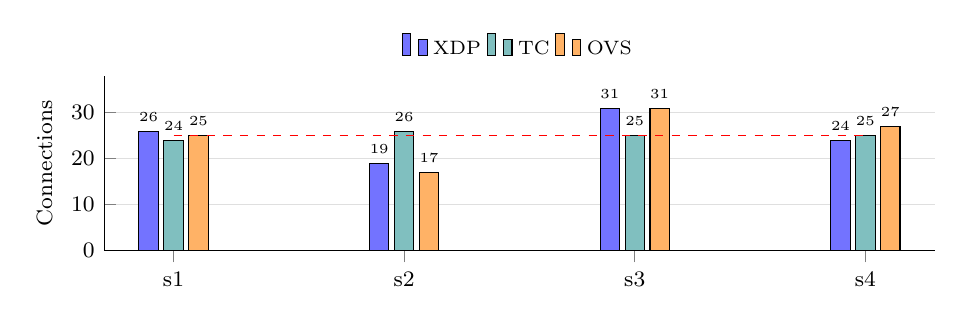
\begin{tikzpicture}
\begin{axis}[ybar, width=\columnwidth, height=3.8cm, bar width=7pt,
  symbolic x coords={s1,s2,s3,s4}, xtick=data, ymin=0, ymax=38,
  ylabel={Connections}, axis lines*=left, ymajorgrids, grid style={gray!25},
  legend style={font=\scriptsize, at={(0.5,1.03)}, anchor=south, legend columns=3, draw=none},
  tick label style={font=\footnotesize}, label style={font=\footnotesize},
  nodes near coords, every node near coord/.append style={font=\tiny}]
\addplot[fill=blue!55] coordinates {(s1,26) (s2,19) (s3,31) (s4,24)};
\addplot[fill=teal!50] coordinates {(s1,24) (s2,26) (s3,25) (s4,25)};
\addplot[fill=orange!60] coordinates {(s1,25) (s2,17) (s3,31) (s4,27)};
\draw[dashed, red] (axis cs:s1,25) -- (axis cs:s4,25);
\legend{XDP, TC, OVS}
\end{axis}
\end{tikzpicture}
\caption{Distribution of 100 new connections to the VIP over four backends
(dashed: ideal 25 per backend).}
\label{fig:dist}
\end{figure}

\subsection{Throughput and Packet Rate}
Table~\ref{tab:perf} lists all measurements, and Fig.~\ref{fig:tput} plots
throughput and packet rate. Plain kernel routing reaches 3.17~Gbit/s of TCP
throughput and 186.6~kpps for 64-byte frames. Relative to it, the eBPF
configurations lose 4.9\% (XDP), 24.9\% (TC) and 8.5\% (TC+FIB) of TCP
throughput and 20.9\%, 25.7\% and 22.6\% of the 64-byte packet rate. OVS
stays within 2\% of plain routing for small packets and reaches the highest
TCP throughput (3.41~Gbit/s). In-program FIB forwarding improves on TC alone
by 21.9\% in TCP throughput and 4.2\% in packet rate, since redirected
packets bypass the kernel's IP routing layer.

\begin{table}[t]
\caption{Benchmark results (path $c_1 \to$ gateway $\to s_2$; one 10-s run each)}
\label{tab:perf}
\centering\scriptsize
\setlength{\tabcolsep}{3pt}
\begin{tabular}{@{}lrrrrr@{}}
\toprule
Metric & XDP & TC & TC+FIB & Kernel & OVS \\
\midrule
TCP throughput (Gbit/s) & 3.02 & 2.38 & 2.90 & 3.17 & 3.41 \\
64-B UDP rate (kpps)    & 147.6 & 138.6 & 144.4 & 186.6 & 183.6 \\
64-B UDP loss (\%)      & 0.71 & 0.00 & 0.07 & 0.07 & 0.08 \\
RTT min / avg (ms)      & .011/.047 & .004/.014 & .004/.023 & .003/.011 & .004/.014 \\
RTT max / mdev (ms)     & .378/.024 & .094/.013 & .185/.024 & .081/.008 & .673/.032 \\
VIP connections/s       & 389.5 & 524.3 & 393.0 & -- & 392.7 \\
VIP request time (ms)   & 2.56 & 1.91 & 2.54 & -- & 2.54 \\
Firewall drops (kpps)   & 230.5 & 277.0 & 240.7 & -- & -- \\
\bottomrule
\end{tabular}
\end{table}

\begin{figure}[t]
\centering
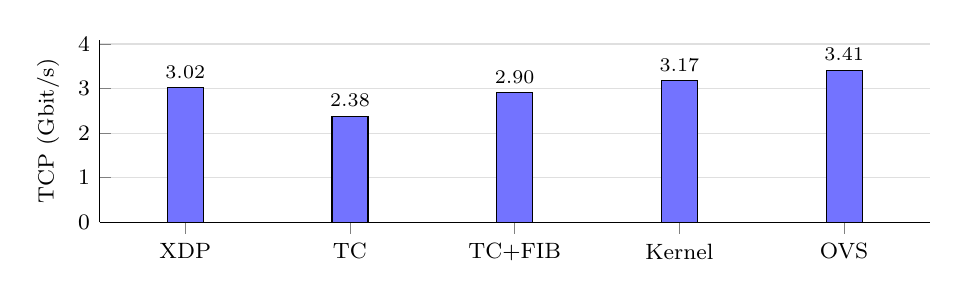
\begin{tikzpicture}
\begin{axis}[benchbar, ylabel={TCP (Gbit/s)}, ymax=4.1,
  every node near coord/.append style={/pgf/number format/fixed, /pgf/number format/fixed zerofill, /pgf/number format/precision=2}]
\addplot[fill=blue!55] coordinates {(XDP,3.017) (TC,2.381) (TC+FIB,2.903) (Kernel,3.172) (OVS,3.411)};
\end{axis}
\end{tikzpicture}\\[1mm]
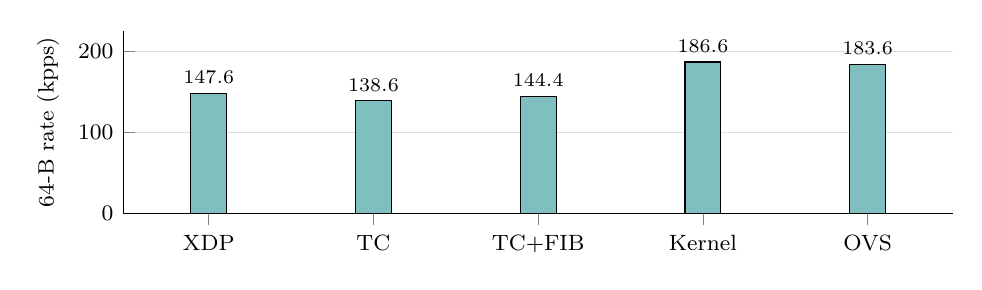
\begin{tikzpicture}
\begin{axis}[benchbar, ylabel={64-B rate (kpps)}, ymax=225,
  every node near coord/.append style={/pgf/number format/fixed, /pgf/number format/precision=1}]
\addplot[fill=teal!50] coordinates {(XDP,147.585) (TC,138.596) (TC+FIB,144.360) (Kernel,186.564) (OVS,183.643)};
\end{axis}
\end{tikzpicture}
\caption{TCP throughput (top) and received 64-byte packet rate (bottom).}
\label{fig:tput}
\end{figure}

\subsection{Latency and Connection Rate}
Fig.~\ref{fig:rtt} shows the RTT. Kernel routing has the lowest average
(0.011~ms). TC and OVS follow at 0.014~ms; OVS has the largest maximum
(0.673~ms) and deviation, which may reflect occasional flow-cache misses
handled in user space. XDP
has the highest average RTT (0.047~ms) and the largest per-packet loss in the
UDP test (0.71\%). The new-connection rate through the VIP is similar for XDP,
TC+FIB and OVS (389--393 connections/s) and highest for TC (524/s); at this
level the rate is dominated by the user-space HTTP client and server rather
than by the gateway.

\begin{figure}[t]
\centering
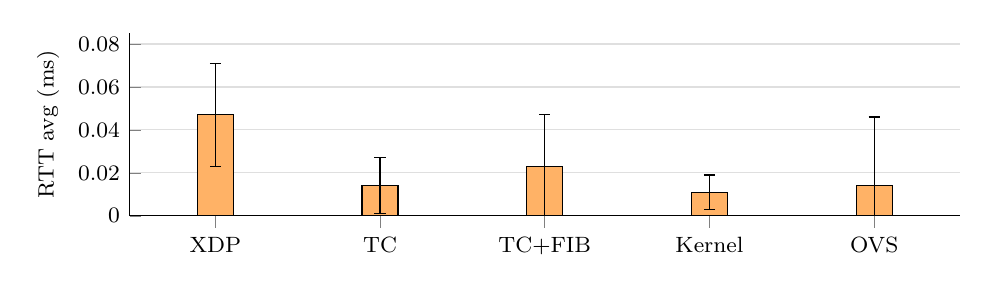
\begin{tikzpicture}
\begin{axis}[benchbar, ylabel={RTT avg (ms)}, ymax=0.085,
  nodes near coords={}, yticklabel style={/pgf/number format/fixed,/pgf/number format/precision=2},
  scaled y ticks=false]
\addplot[fill=orange!60, error bars/.cd, y dir=both, y explicit]
  coordinates {(XDP,0.047) +- (0,0.024) (TC,0.014) +- (0,0.013) (TC+FIB,0.023) +- (0,0.024)
               (Kernel,0.011) +- (0,0.008) (OVS,0.014) +- (0,0.032)};
\end{axis}
\end{tikzpicture}
\caption{Average round-trip time; error bars show the mean deviation
(\texttt{ping} mdev) over 500 echoes.}
\label{fig:rtt}
\end{figure}

\subsection{In-Kernel Filtering}
During the 3-s floods, every datagram sent toward the blocked port was dropped
by the eBPF program (721\,408 of 721\,408 at XDP, 861\,952 of 861\,952 at TC,
765\,952 of 765\,952 at TC+FIB), i.e., 230--277~kpps. These rates equal the
sender's rate: a single-threaded Python generator could not saturate the
filter, so they are lower bounds on the drop capacity.

\subsection{Discussion}
The results separate two properties. \emph{Functionally}, the eBPF data
plane is strictly more capable than the OpenFlow~1.3 baseline: it tracks
connections, rewrites only replies that belong to load-balanced connections,
re-places connections of drained backends, and exports per-flow counters,
while matching it in reachability, filtering and load balance.
\emph{Performance-wise}, on veth links it is slower than plain routing and
OVS. Two causes explain this. First, XDP's advantage comes from running in the
NIC driver before a socket buffer is allocated; a veth packet already has one,
so native veth XDP must convert it to an XDP buffer and back and forgoes
receive aggregation, which adds work instead of saving it---visible as XDP's
higher RTT. Second, the eBPF configurations perform policy work on every
packet (parsing, up to nine rule lookups, connection-table and telemetry
updates), whereas the kernel baseline performs none. FIB forwarding recovers
part of the gap by skipping the routing layer, as Fig.~\ref{fig:tput} shows.

\subsection{Threats to Validity}
\label{sec:threats}
Each configuration was measured once for 10~s on a laptop CPU with dynamic
frequency scaling, so differences of roughly 10--20\% are within the
run-to-run variation one should expect; only the larger gaps (e.g., eBPF
versus kernel/OVS at 64~bytes) should be interpreted. All links are veth
pairs inside one machine, which, as discussed, does not exercise XDP's
driver-level fast path. Traffic generators (\texttt{iperf3}, Python) run on the
same CPU as the gateway. Finally, the OVS baseline's reverse NAT is stateless,
so it performs less work per packet than a conntrack-based OVS configuration
would.

%=====================================================================
\section{Conclusion}
%=====================================================================
We designed, implemented and evaluated an eBPF/XDP data plane that moves the
SDN switch into the Linux kernel. One verified pipeline provides a stateful
firewall, an L4 load balancer with DNAT/SNAT and $O(1)$ incremental checksum
maintenance, and per-flow telemetry at either the XDP or the TC hook, while a
libbpf-based control plane reprograms it at runtime and expires connection
state like OpenFlow timeouts. The implementation passes 69 automated tests and
all end-to-end scenarios at both hooks, spreads connections uniformly
($p \ge 0.25$), and supports connection tracking and backend draining that the
OpenFlow~1.3 baseline cannot express. On emulated veth links it forwards
2.4--3.0~Gbit/s and 139--148~kpps, about 21--26\% below plain kernel routing,
because veth links do not benefit from XDP's driver-level execution. Future
work will evaluate the system on physical NICs with native XDP support and
hardware traffic generators with repeated runs, replace modulo hashing with
consistent hashing such as Maglev \cite{eisenbud2016maglev} to reduce
connection remapping when pools change, and add prefix-based (LPM) firewall
rules.

%=====================================================================
\begin{thebibliography}{00}
\bibitem{kreutz2015sdn} D. Kreutz, F. M. V. Ramos, P. E. Ver\'issimo,
C. E. Rothenberg, S. Azodolmolky, and S. Uhlig, ``Software-defined networking:
A comprehensive survey,'' \textit{Proc. IEEE}, vol.~103, no.~1, pp.~14--76,
Jan. 2015.

\bibitem{feamster2014road} N. Feamster, J. Rexford, and E. Zegura, ``The road
to SDN: An intellectual history of programmable networks,'' \textit{ACM
SIGCOMM Comput. Commun. Rev.}, vol.~44, no.~2, pp.~87--98, Apr. 2014.

\bibitem{mckeown2008openflow} N. McKeown \textit{et al.}, ``OpenFlow: Enabling
innovation in campus networks,'' \textit{ACM SIGCOMM Comput. Commun. Rev.},
vol.~38, no.~2, pp.~69--74, Apr. 2008.

\bibitem{pfaff2015ovs} B. Pfaff \textit{et al.}, ``The design and
implementation of Open vSwitch,'' in \textit{Proc. 12th USENIX Symp. Netw.
Syst. Design Implement. (NSDI)}, Oakland, CA, USA, 2015, pp.~117--130.

\bibitem{hoiland2018xdp} T. H{\o}iland-J{\o}rgensen \textit{et al.}, ``The
eXpress data path: Fast programmable packet processing in the operating system
kernel,'' in \textit{Proc. 14th Int. Conf. Emerg. Netw. Exp. Technol.
(CoNEXT)}, Heraklion, Greece, 2018, pp.~54--66.

\bibitem{vieira2020ebpf} M. A. M. Vieira \textit{et al.}, ``Fast packet
processing with eBPF and XDP: Concepts, code, challenges, and applications,''
\textit{ACM Comput. Surv.}, vol.~53, no.~1, Art. no.~16, Feb. 2020.

\bibitem{cilium} Cilium Authors, ``Cilium: eBPF-based networking,
observability, and security.'' [Online]. Available: https://cilium.io

\bibitem{katran} Meta Platforms, ``Katran: A high performance layer 4 load
balancer.'' [Online]. Available: https://github.com/facebookincubator/katran

\bibitem{bosshart2014p4} P. Bosshart \textit{et al.}, ``P4: Programming
protocol-independent packet processors,'' \textit{ACM SIGCOMM Comput. Commun.
Rev.}, vol.~44, no.~3, pp.~87--95, Jul. 2014.

\bibitem{miano2018creating} S. Miano, M. Bertrone, F. Risso, M. Tumolo, and
M. V. Bernal, ``Creating complex network services with eBPF: Experience and
lessons learned,'' in \textit{Proc. IEEE 19th Int. Conf. High Perform. Switching
Routing (HPSR)}, Bucharest, Romania, 2018, pp.~1--8.

\bibitem{scholz2018filtering} D. Scholz, D. Raumer, P. Emmerich, A. Kurtz,
K. Lesiak, and G. Carle, ``Performance implications of packet filtering with
Linux eBPF,'' in \textit{Proc. 30th Int. Teletraffic Congr. (ITC)}, Vienna,
Austria, 2018, pp.~209--217.

\bibitem{eisenbud2016maglev} D. E. Eisenbud \textit{et al.}, ``Maglev: A fast
and reliable software network load balancer,'' in \textit{Proc. 13th USENIX
Symp. Netw. Syst. Design Implement. (NSDI)}, Santa Clara, CA, USA, 2016,
pp.~523--535.

\bibitem{lantz2010mininet} B. Lantz, B. Heller, and N. McKeown, ``A network in
a laptop: Rapid prototyping for software-defined networks,'' in \textit{Proc.
9th ACM SIGCOMM Workshop Hot Topics Netw. (HotNets)}, Monterey, CA, USA, 2010,
Art. no.~19.

\bibitem{rfc1624} A. Rijsinghani, ``Computation of the Internet checksum via
incremental update,'' RFC 1624, IETF, May 1994.

\bibitem{rfc1071} R. Braden, D. Borman, and C. Partridge, ``Computing the
Internet checksum,'' RFC 1071, IETF, Sep. 1988.
\end{thebibliography}

\end{document}
